\documentclass[12pt,letterpaper]{article}
\usepackage{fullpage}
\usepackage[top=1.5cm, bottom=3.5cm, left=2.2cm, right=2.2cm]{geometry}
\usepackage{amsmath,amsthm,amsfonts,amssymb,amscd, esint}
\usepackage{lastpage}
\usepackage{enumerate}
\usepackage{fancyhdr}
\usepackage{mathrsfs}
\usepackage{graphicx}
\usepackage{listings}
\usepackage{hyperref}
\usepackage[english]{babel}
\usepackage{emoji}
\usepackage{lipsum}
\usepackage{braket}
\usepackage[table,xcdraw]{xcolor}
\usepackage{enumitem}
\usepackage{float}
\usepackage{chemfig}
\usepackage{yfonts}
\usepackage{tikz}
\usepackage{wrapfig}
\usepackage{url}
\usepackage{natbib}
\usepackage[normalem]{ulem}
\usepackage{multicol}
\useunder{\uline}{\ul}{}


%%%%%%%%%%%%%%% CODELISTINGS %%%%%%%%%%%%%%%%
\usepackage{listings}
\definecolor{codegreen}{rgb}{0,0.6,0}
\definecolor{codegray}{rgb}{0.5,0.5,0.5}
\definecolor{codepurple}{rgb}{0.58,0,0.82}
\definecolor{backcolour}{rgb}{0.95,0.95,0.92}

\lstdefinestyle{mystyle}{
    backgroundcolor=\color{backcolour},   
    commentstyle=\color{codegreen},
    keywordstyle=\color{magenta},
    numberstyle=\tiny\color{codegray},
    stringstyle=\color{codepurple},
    basicstyle=\ttfamily\footnotesize,
    breakatwhitespace=false,         
    breaklines=true,                 
    captionpos=t,                    
    keepspaces=true,                 
    numbers=left,                    
    numbersep=5pt,                  
    showspaces=false,                
    showstringspaces=false,
    showtabs=false,                  
    tabsize=2
}

\lstset{style=mystyle}

%%%%%%%%%%%%%%%%%%%%%%%%%%%%%%%%%%%%%%% 




\newtheorem{definition}{Definition}
\newtheorem{observation}{Observation}
\newtheorem{reflection}{Reflection}
\newtheorem{PyPackage}{Package}
\newtheorem{book}{Book}

\newcommand{\HRule}[1]{\rule{\linewidth}{#1}}
\setcounter{tocdepth}{5}
\setcounter{secnumdepth}{5}

\setlength{\parindent}{0.0in}
\setlength{\parskip}{0.05in}

% Edit these as appropriate
\newcommand\course{}
\newcommand\subject{Final Degree Project}
\newcommand\degree{Bachelor's Degree in Physics}
\newcommand\documenttitle{Notes: Quantum State Exclusion - Temporal Name -}
\newcommand\NetIDb{Universitat Autònoma de Barcelona}


\begin{document}
\title{\vspace{4cm} \normalsize 
		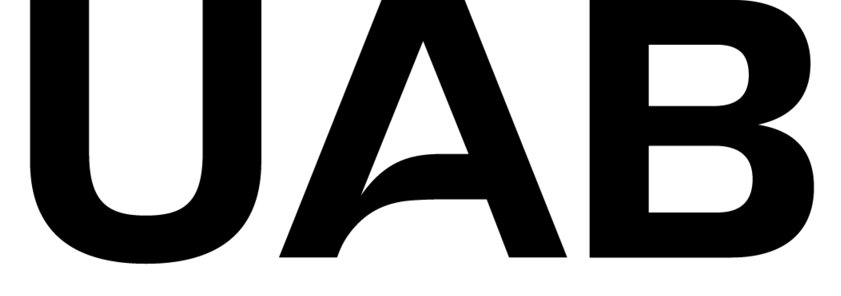
\includegraphics[width = 0.25\textwidth]{GeneralSources/UABLogo.png}\\ [0.5cm]
		\textsc{\NetIDb}\\ [2.0cm]
		\HRule{0.5pt} \\
		\LARGE \textbf{\uppercase{\documenttitle}}
		\HRule{2pt} \\ [1.5cm]
		\normalsize \begin{tabular}{rcl}  % Create a right-left column alignment
        \textsc{Author} & : & \textsc{Sergio Castañeiras Morales} \\
        \textsc{Supervisor} & : & \textsc{Ramón Muñoz Tapia} \\
        \textsc{Co-Supervisor} & : & \textsc{Santiago Llorens Fernández}
    \end{tabular}
    \normalsize \vspace*{5\baselineskip}
		}

\date{2024-2025}

\author{\large \textsc{\subject} \\ \textsc{\degree}}

\begin{titlepage}
\clearpage\maketitle
\thispagestyle{empty}
\end{titlepage}

\newpage
\thispagestyle{empty}
\vspace*{\fill} % Push content to vertical center
\begin{flushright}
    \emph{“The dumbest people I know are those who know it all.”}\\[1em]
    \textbf{Malcolm S. Forbes}
\end{flushright}
\vspace*{\fill} % Balance vertical spacing

\newpage
\pagestyle{fancyplain}
\headheight 35pt
\lhead{\NetIDb}    
\rhead{\subject}
\cfoot{}
\rfoot{\small\thepage}
\headsep 1.5em

%%%%%%%%%%%%%%%%%%%%%%%%%%%%%%%%%%%%%%%%%%
%%%%%%%%%%%%%%%%% DEFINITIONS %%%%%%%%%%%%%%%%%
%%%%%%%%%%%%%%%%%%%%%%%%%%%%%%%%%%%%%%%%%%

\begin{multicols}{2}
[
\section{Definitions}
]
\begin{definition}
\textbf{Completely positive map}: "Let $ A $ and $ B $ be C*-algebras. A linear map $ \phi: A \to B $ is called a \textit{positive map} if $ \phi $ maps positive elements to positive elements:
\begin{align}
a \geq 0 \implies \phi(a) \geq 0.
\end{align}

Any linear map $ \phi: A \to B $ induces another map
\begin{align}
\mathrm{id} \otimes \phi : \mathbb{C}^{k \times k} \otimes A \to \mathbb{C}^{k \times k} \otimes B
\end{align}
in a natural way. If $ \mathbb{C}^{k \times k} \otimes A $ is identified with the C*-algebra $ A^{k \times k} $ of $ k \times k $-matrices with entries in $ A $, then $ \mathrm{id} \otimes \phi $ acts as
\begin{align}
\begin{pmatrix}
a_{11} & \cdots & a_{1k} \\
\vdots & \ddots & \vdots \\
a_{k1} & \cdots & a_{kk}
\end{pmatrix}
\mapsto
\begin{pmatrix}
\phi(a_{11}) & \cdots & \phi(a_{1k}) \\
\vdots & \ddots & \vdots \\
\phi(a_{k1}) & \cdots & \phi(a_{kk})
\end{pmatrix}.
\end{align}

The map $ \phi $ is called \textit{k-positive} if $ \mathrm{id}_{\mathbb{C}^{k \times k}} \otimes \phi $ is a positive map, and \textit{completely positive} if $ \phi $ is $ k $-positive for all $ k $."\cite{completely_positive_map_Wikipedia}
\end{definition}
\begin{definition}\textbf{Kraus operator: } 
\end{definition}

\begin{definition}\label{innerProductDefinition}
\textbf{Inner product}: Given a vector space $A$ and a field $F$ we define the an inner product $\langle \cdot , \cdot \rangle$ as $\langle \cdot , \cdot \rangle:A\times A\rightarrow F$ that satisfies the following properties. Given $x,y,z\in A$ and $\lambda,\mu\in F$:
\begin{enumerate}
\item Conjugate symmetry: $\langle x,y\rangle=(\langle y,x\rangle)^*$.
\item Linearity: $\langle \lambda x+\mu y, z\rangle=\lambda\langle  x, z\rangle+\mu\langle  y, z\rangle$
\item Positive-definiteness: $\langle x,x\rangle>0$ if $x\neq0$
\end{enumerate}
\end{definition}

\begin{definition}
\textbf{Inner product space}: Given a vector space $A$ and a field $F$ we define the  inner product space as the duple $(A,\langle \cdot , \cdot \rangle)$ such that  $\langle \cdot , \cdot \rangle:A\times A\rightarrow F$ is an inner product.
\end{definition}

\begin{definition}\label{defGramMatrix}
\textbf{Gram matrix}: Given a vector space $A$, a field $F$ , a set of vectors $\{v_i\}_{i=0}^n\subset A$ and an inner product space such that  $\langle \cdot , \cdot \rangle:A\times A\rightarrow F$  the Gram matrix $G$ is defined as the matrix $G\in F^{n\times n}$ whose entries are $g_{i,j}=\langle v_i,v_j\rangle$ i.e,
\begin{align}
G=\begin{pmatrix}
\langle v_1,v_1\rangle & \hdots & \langle v_1,v_n\rangle\\
\vdots & \ddots & \vdots\\
\langle v_n,v_1\rangle & \hdots & \langle v_n,v_n\rangle
\end{pmatrix}.
\end{align}
Due to the first property of the inner product definition \ref{innerProductDefinition} it is immediate that $G^\dagger =G$ in other word G is hemitian (trivial proof).
\end{definition}

\end{multicols}
\newpage

\begin{multicols}{2}
\begin{observation}
Let $\mathcal{U}$ be a unitary matrix such that $\mathcal{U}^n=\mathbb{I}_d$ and $\mathcal{U}^i\neq\mathbb{I}_d\;\;\forall i\in\{0,...,n-1\}$, let $\ket{\psi}$ also be a normalised state. We might define the set of quantum states $\Omega=\{\ket{\psi_i}=\mathcal{U}^i\ket{\psi}\}_{i=0}^{n-1}$ a group generated ensamble of states, since the set  $\{\mathcal{U}^i\}_{i=0}^{n-1}$ is obviously a group with the usual product. From the group structure of $\{\mathcal{U}^i\}_{i=0}^{n-1}$ it is natural to define $\star$ operation such that,
\begin{align}
\star:\Omega\times\Omega\rightarrow&\Omega\\
(\ket{\psi_i},\ket{\psi_j})\mapsto&\ket{\psi_{i+j}}.
\end{align}
Hence we observe the ensamble of states inherites the group structure from the generator $\mathcal{U}$ nature. More particularly, $\Omega$ is isomorphic to $\mathbb{Z}/n\mathbb{Z}$. Hence we want to compute the gram matrix of $\Omega$, applying the Definition (\ref{defGramMatrix}) we obtain,
\begin{align}
G_{i,j} =& \braket{\psi_{i}|\psi_{j}} \\
=& \bra{\psi} \left(\mathcal{U}^i\right)^\dagger U^j\ket{\psi}\\
=& \bra{\psi} \left(\mathcal{U}^\dagger\right)^i U^j\ket{\psi}\\
=& \bra{\psi} \left(\mathcal{U}^{-1}\right)^i U^j\ket{\psi}\\
=& \bra{\psi} \mathcal{U}^{-i} U^j\ket{\psi}\\
=& \braket{\mathcal{U}^{-i+j}}_\psi.
\end{align}
The gram matrix must have the shape
\begin{align}
G=\begin{pmatrix}
 1 & \braket{\mathcal{U}^{1}}_{\psi} & \hdots &  \braket{\mathcal{U}^{n-1}}_{\psi} \\
  \braket{\mathcal{U}^{-1}}_{\psi} & 1 & \hdots &  \braket{\mathcal{U}^{n-2}}_{\psi} \\
   \vdots & \vdots & \ddots & \vdots \\
  \braket{\mathcal{U}^{-n+1}}_{\psi} & \braket{\mathcal{U}^{-n+2}}_{\psi}  & \hdots &  1
\end{pmatrix}.
\end{align}
Since $\braket{\mathcal{U}^{-j}}_{\psi}=\braket{\mathcal{U}^{j}}_{\psi}^*$ the hermicity is preserved (as it should). Also we note that,
\begin{align}
\braket{\mathcal{U}^{-n+i}}_{\psi}=\braket{\mathcal{U}^{-n+i}\mathbb{I}_d}_{\psi}=\braket{\mathcal{U}^{-n+i}\mathcal{U}^{n}}_{\psi}=\braket{\mathcal{U}^{i}}_{\psi}
\end{align}
hence,
\begin{align}
G=\begin{pmatrix}
 1 & \braket{\mathcal{U}}_{\psi} & \braket{\mathcal{U}^{2}}_{\psi} & \hdots &  \braket{\mathcal{U}}_{\psi}^* \\
  \braket{\mathcal{U}}_{\psi}^* & 1 & \braket{\mathcal{U}}_{\psi} & \hdots &  \braket{\mathcal{U}^{2}}_{\psi}^* \\
    \braket{\mathcal{U}^{2}}_{\psi}^* &  \braket{\mathcal{U}}_{\psi}^*  & 1 & \hdots &  \braket{\mathcal{U}^{3}}_{\psi}^* \\
   \vdots & \vdots & \vdots & \ddots & \vdots \\
  \braket{\mathcal{U}}_{\psi} & \braket{\mathcal{U}^{2}}_{\psi}  & \braket{\mathcal{U}^{3}}_{\psi}  & \hdots &  1 
\end{pmatrix}.
\end{align}
\textbf{Question} how does $\braket{\mathcal{U}^{j}}_{\psi}$ depend on $\braket{\mathcal{U}}_{\psi}$. I know we have said $\braket{\mathcal{U}^{j}}_{\psi} =\braket{\mathcal{U}}_{\psi}$ but I cannot see why \emoji{sad-but-relieved-face}\par
As a matter of fact by computing some matrices I can get situations such that $\braket{\mathcal{U}^{i}}_{\psi}=0$ for instance by performing a rotation of $\pi/4$ in the $x$ axis of the state pointing in the $z$ direction I can get a group generated ensamble of $\mathbb{Z}/4\mathbb{Z}$. But the second state (rotation of $\pi/2$) is orthogonal to the first state and $\braket{\mathcal{U}^2}_{\psi}=0\neq \frac{1}{\sqrt{2}}\braket{\mathcal{U}}_{\psi}$. \par
\textbf{Stuff I know},\par 
Since $\mathcal{U}$ is an unitary matrix such that $\mathcal{U}^n=\mathbb{I}_d$ I know that in the basis of eigenvalues of $\mathcal{U}$ denoted as $\{\ket{u_i}\}_{i=0}^{n-1}$
\begin{align}
\mathcal{U}=\sum_{k=0}^{n-1}e^{i2\pi k/n}\ket{u_k}\bra{u_k}
\end{align}
Let $\ket{\psi}=\sum_{i=0}^{n-1}c_i\ket{u_i}$ be the expression of $\ket{\psi}$ in the $\{\ket{u_i}\}_{i=0}^{n-1}$ basis. Notice from the unicity of $\mathcal{U}$ can be expressed as $\mathcal{U}=e^{iA}$ for a hermitian matrix $A$, which decomposes in the basis orthonormal basis as $A=\sum_{i=0}^{n-1}\alpha_i\ket{a_i}\bra{a_i}$. Therefore,
\begin{align}
\mathcal{U}=&e^{iA}\\
=&\sum_{j=0}^{\infty}\frac{i^j}{j!}A^j\\
=&\sum_{j=0}^{\infty}\frac{i^j}{j!}\left(\sum_{k=0}^{n-1}\alpha_k\ket{a_k}\bra{a_k}\right)^j\\
=&\sum_{j=0}^{\infty}\frac{i^j}{j!}\sum_{k=0}^{n-1}\alpha_k^j\ket{a_k}\bra{a_k}\\
=&\sum_{k=0}^{n-1}\left(\sum_{j=0}^{\infty}\frac{i^j}{j!}\alpha_k^j\right)\ket{a_k}\bra{a_k}\\
=&\sum_{k=0}^{n-1}e^{i\alpha_k}\ket{a_k}\bra{a_k}
\end{align}
here we deduce 
\begin{align}
\ket{u_k}=&\ket{a_k}\\
2\pi k/n =& \alpha_k\\
A=&\frac{2\pi}{n}\sum_{i=0}^{n-1}i \ket{a_i}\bra{a_i}\\
\ket{\psi}=&\sum_{i=0}^{n-1}c_i\ket{a_i}.
\end{align}
Then we might compute $\braket{\mathcal{U}}_\psi$ as,
\begin{align}
\braket{\mathcal{U}}_\psi= \sum_{k=0}^{n-1}|c_i|^2e^{i2\pi k/n}
\end{align}
which is not necessarily a real quantity, then we compute $\braket{\mathcal{U}^j}_\psi$ as
\begin{align}
\braket{\mathcal{U}^j}_\psi= \sum_{k=0}^{n-1}|c_k|^2e^{i2\pi kj/n}
\end{align}
The basis we knew the gram matrix decompose in \emoji{star-struck} (the Fourier's basis), it is a genuine surprise I did not expect this result. Then the Gram matrix can be written as,
\end{observation}
\end{multicols}
\begin{align}
G=\begin{pmatrix}
 1 & \sum_{k=0}^{n-1}|c_k|^2e^{i2\pi k/n} & \sum_{k=0}^{n-1}|c_k|^2e^{i4\pi k/n}  & \hdots &  \sum_{k=0}^{n-1}|c_k|^2e^{-i2\pi k/n} \\
  \sum_{k=0}^{n-1}|c_k|^2e^{-i2\pi k/n} & 1 & \sum_{k=0}^{n-1}|c_k|^2e^{-i2\pi k/n} & \hdots & \sum_{k=0}^{n-1}|c_k|^2e^{-i4\pi k/n} \\
   \sum_{k=0}^{n-1}|c_k|^2e^{-i4\pi k/n} &  \sum_{k=0}^{n-1}|c_k|^2e^{-i2\pi k/n}  & 1 & \hdots & \sum_{k=0}^{n-1}|c_k|^2e^{-i6\pi k/n} \\
   \vdots & \vdots & \vdots & \ddots & \vdots \\
  \sum_{k=0}^{n-1}|c_k|^2e^{i2\pi k/n} &\sum_{k=0}^{n-1}|c_k|^2e^{i4\pi k/n}  & \sum_{k=0}^{n-1}|c_k|^2e^{i6\pi k/n}  & \hdots &  1 
\end{pmatrix}.
\end{align}
\begin{multicols}{2}
\begin{observation}
We can immediately see the gram matrix is completely determined by the decomposition of $\ket{\psi}$ in the basis of eigenvectors of $A$ i.e. $\mathcal{U}$ but the statement $\braket{\mathcal{U}^{j}}_{\psi} =\braket{\mathcal{U}}_{\psi}$ still remains untrue in general. \par 
An interesting case can be $\ket{\psi}=\ket{a_t}$ for a given $t\in\{0,..,n-1\}$. In this case we can see that 
\begin{align}
U^j\ket{\psi}&=U^j\ket{a_t}\\&=e^{i2\pi t/n}\ket{a_t}\\&=e^{i2\pi t/n}\ket{\psi}
\end{align}
In this case the gram matrix is
\end{observation}
\end{multicols}
\begin{align}\label{eqGramMatrixZn}
G=\begin{pmatrix}
 1 & |c_t|^2e^{i2\pi t/n} & |c_t|^2e^{i4\pi t/n} & \hdots &  |c_t|^2e^{-i2\pi t/n} \\
  |c_t|^2e^{-i2\pi t/n} & 1 & |c_t|^2e^{i2\pi t/n} & \hdots & |c_t|^2e^{-i4\pi t/n} \\
  |c_t|^2e^{i4\pi t/n} &  |c_t|^2e^{-i2\pi t/n}  & 1 & \hdots & |c_t|^2e^{-i6\pi t/n}  \\
   \vdots & \vdots & \vdots & \ddots & \vdots \\
  |c_t|^2e^{i2\pi t/n} &|c_t|^2e^{i4\pi t/n}  & |c_t|^2e^{i6\pi t/n}  & \hdots &  1 
\end{pmatrix}
\end{align}

\begin{multicols}{2}
\begin{observation}
Still we need to get rid off the global phase in each entry to get the result explain in the meetings... \par
\textbf{Question} Which is the criteria to do this? Why can we choose $\ket{\psi}$ to be an eigenket of $A$ arbitrarily? Regarding the previous example we had our state pointing in the $z$ direction (i.e. not an eigenket of $\sigma_x$) which would explain the inconsistency.
\end{observation}
\begin{observation}
Let us analyse the case of the group generated ensemble of $\mathbb{Z}/2\mathbb{Z}\times\mathbb{Z}/2\mathbb{Z}$. We will denote 
\end{observation}
\begin{observation}\label{ObsZnZm}
Let us analyse the case the case $\mathbb{Z}/n\mathbb{Z}\times\mathbb{Z}/m\mathbb{Z}$ in order to do so let $\mathcal{U}_n$ and $\mathcal{U}_m$ two unitary operators such that $\mathcal{U}_n^n=\mathbb{I}_d$, $\mathcal{U}_m^m=\mathbb{I}_d$ respectively, and $[U_n,U_m]=0$. Here we distinguish two cases $n=m$ and $n\neq m$. Since $[U_n,U_m]=0$ we know there exists a basis $\{\ket{u}_i\}_{i=0}^{nm-1}$ where both unitary operators are diagonal. Taking into account the group representations are equivalent up to isomorphism we can consider one representation and extend it to any other representation. Here we might consider,
\begin{align}
U_n=&\sum_{i=0}^{nm-1}e^{i2\pi i/n}\ket{u_i}\bra{u_i}\\
U_m=&\sum_{i=0}^{nm-1}e^{i2\pi i/m}\ket{u_i}\bra{u_i}
\end{align}
Notice the rellevance $n\neq m\Rightarrow U_n\neq U_m$ otherwise the states generated by $U_n$ and $U_m$ will be the same ones and we would go back to the case $\mathbb{Z}/n\mathbb{Z}$. \emoji{thinking-face}\par
Now our set of states is $\Omega=\{U_{n}^iU_{m}^j\ket{\psi}\}_{0\leq i\leq n-1; 0\leq j\leq m-1}$ without loss of generality and for notation purposes we will choose $n>m$ and denote $U_{n}^iU_{m}^j\ket{\psi}=\ket{\psi_{(i,j)}}$ and we will define the oder relation \footnote{We need to order our ensemble for generating the gram matrix.},
\begin{align}
\ket{\psi_{(i,j)}}=&\ket{\psi_{(k,l)}}\Leftrightarrow i=k\;\&\;j=k\\
\ket{\psi_{(i,j)}}>&\ket{\psi_{(k,l)}}\Leftrightarrow\begin{cases}i>k\\i=k\;\&\;j>k\end{cases}\\
\ket{\psi_{(i,j)}}<&\ket{\psi_{(k,l)}}\Leftrightarrow\begin{cases}i<k\\i=k\;\&\;j<k\end{cases}
\end{align}
now we have $\Omega$ ready to compute the gram matrix. Let $G_m$ be the gram matrix of the $\mathbb{Z}/m\mathbb{Z}$ group generated from Eq.(\ref{eqGramMatrixZn}), then the gram matrix is nothing but,
\end{observation}
\end{multicols}
\begin{align}\label{EqGramZnZm}
G_{nm}=\begin{pmatrix}
 G_m & G_me^{i2\pi t/n} & G_me^{i4\pi t/n} & \hdots &  G_me^{-i2\pi t/n} \\
  G_me^{-i2\pi t/n} & G_m & G_me^{i2\pi t/n} & \hdots & G_me^{-i4\pi t/n} \\
  G_me^{i4\pi t/n} &  G_me^{-i2\pi t/n}  & G_m & \hdots & G_me^{-i6\pi t/n}  \\
   \vdots & \vdots & \vdots & \ddots & \vdots \\
  G_me^{i2\pi t/n} &G_me^{i4\pi t/n}  & G_me^{i6\pi t/n}  & \hdots &  G_m 
\end{pmatrix}
\end{align}

\begin{multicols}{2}
\begin{observation}
Notice by changing the ordering definition we can easily see $G_{nm}$ is totally equivalent to $G_{mn}$ since $\mathbb{Z}/n\mathbb{Z}\times\mathbb{Z}/m\mathbb{Z}\equiv \mathbb{Z}/m\mathbb{Z}\times\mathbb{Z}/n\mathbb{Z}$ naturally. From Observation (\ref{ObsZnZm}) and Eq. (\ref{EqGramZnZm}) one can deduce, for the case $\mathbb{Z}/n_1\mathbb{Z}\times\mathbb{Z}/n_2\mathbb{Z}\times\dots\times \mathbb{Z}/n_k\mathbb{Z}$, the gram matrix in nothing but,
\end{observation}
\end{multicols}
\begin{align}
G_{n_1,n_2,...,n_k}=\begin{pmatrix}
 G_{n_1,n_2,...,n_{k-1}} & G_{n_1,n_2,...,n_{k-1}}e^{i2\pi t/n_k} & \hdots &  G_{n_1,n_2,...,n_{k-1}}e^{-i2\pi t/n_k} \\
  G_{n_1,n_2,...,n_{k-1}}e^{-i2\pi t/n_k} & G_{n_1,n_2,...,n_{k-1}} & \hdots & G_{n_1,n_2,...,n_{k-1}}e^{-i4\pi t/n_k} \\
   \vdots & \vdots  & \ddots & \vdots \\
  G_{n_1,n_2,...,n_{k-1}}e^{i2\pi t/n_k} & G_{n_1,n_2,...,n_{k-1}}e^{i4\pi t/n_k}  & \hdots &  G_{n_1,n_2,...,n_{k-1}} 
\end{pmatrix}.
\end{align}

\newpage

%%%%%%%%%%%%%%%%%%%%%%%%%%%%%%%%%%%%%%%%%%
%%%%%%%%%%%%%%%% BIBLIOGRAPHY %%%%%%%%%%%%%%%%%
%%%%%%%%%%%%%%%%%%%%%%%%%%%%%%%%%%%%%%%%%%

\bibliographystyle{plain}
\bibliography{references} 
%%%%%%%%


\end{document}